\documentclass[main.tex]{subfiles}

\begin{document}

\section{Deskriptívna analýza}
Ako prvé sa pozrieme na základné štatistické ukazovatele pre obe železničné siete – slovenskú aj českú. Obe tieto siete môžeme vidieť na obrázkoch \ref{obr:1} a \ref{obr:2}.
\begin{figure}
    \centerline{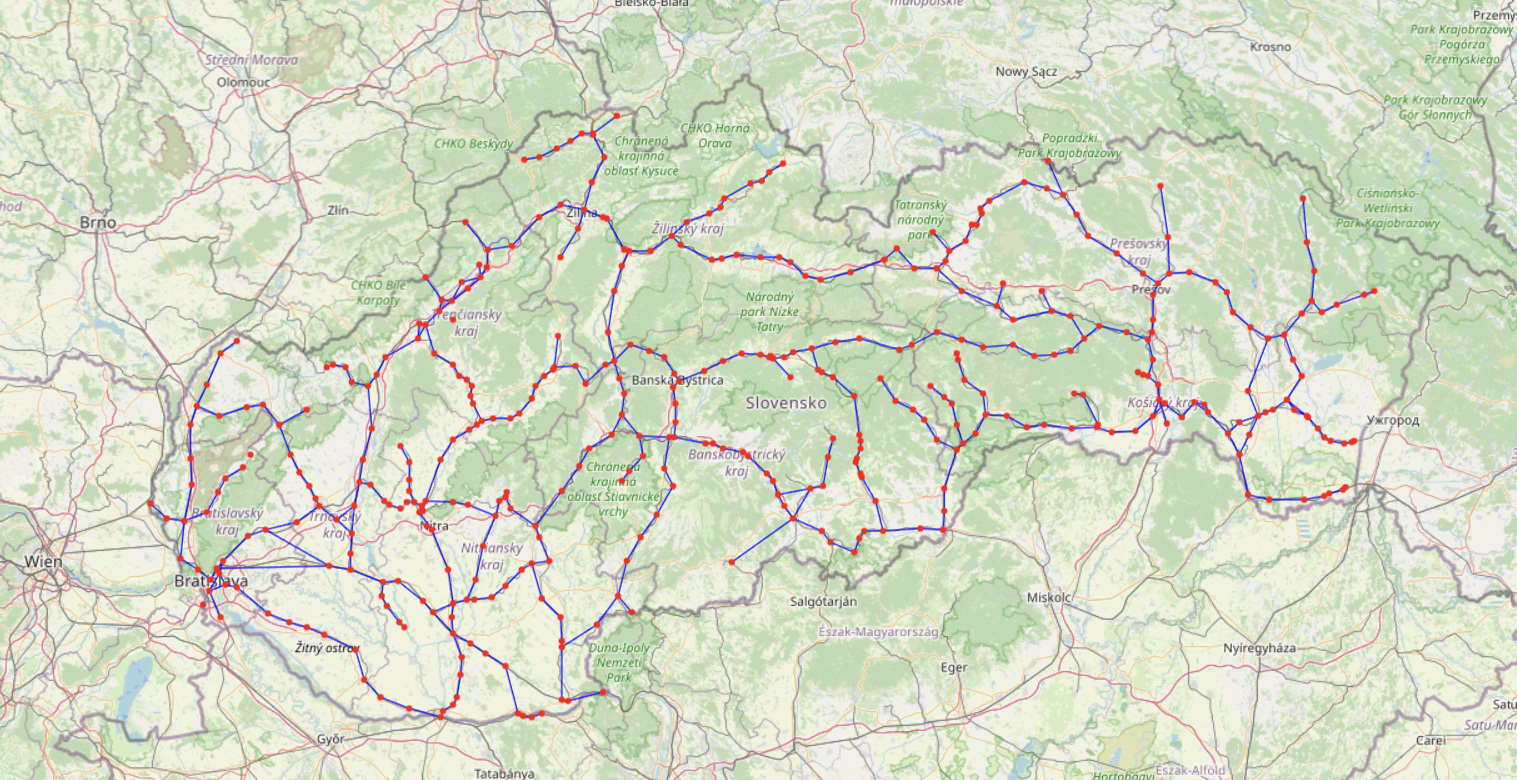
\includegraphics[width=1\textwidth]{images/sk_railroads.png}}
    \caption{Železničná trať Slovenska}
    \label{obr:1}
\end{figure}

\begin{figure}
    \centerline{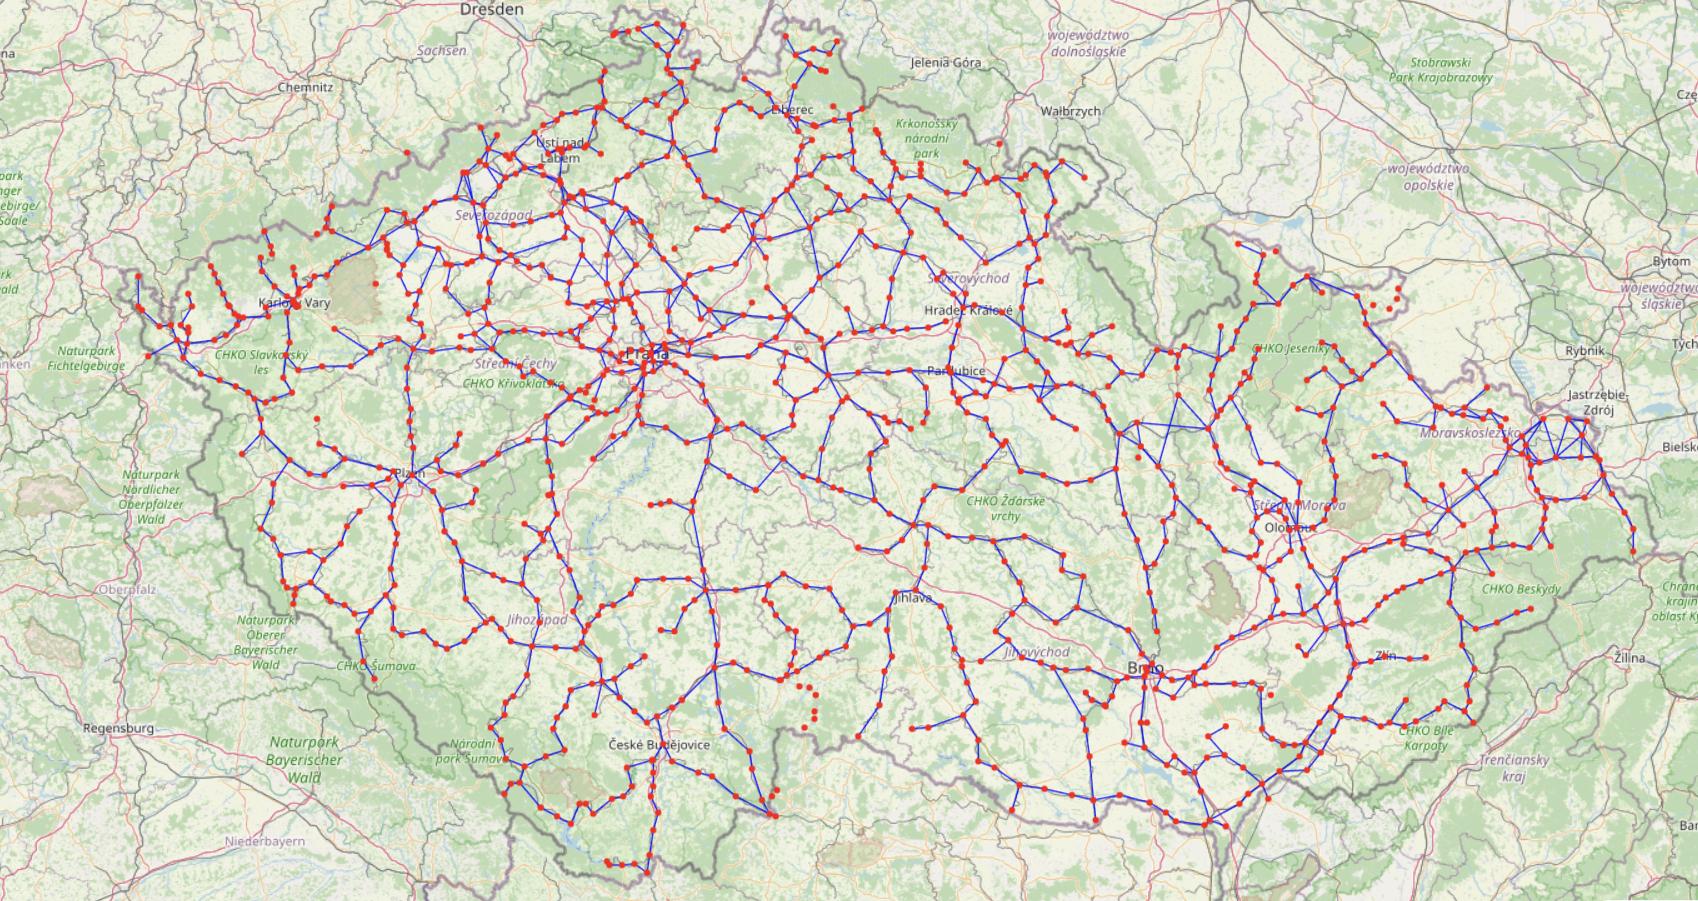
\includegraphics[width=1\textwidth]{images/cze_railroads.png}}
    \caption{Železničná trať Česka}
    \label{obr:2}
\end{figure}


Okrem iných metrík uvádzame aj vážený polomer a vážený priemer grafu (tzv. diameter), ktoré bližšie charakterizujú štruktúru siete z hľadiska vzdialeností medzi stanicami.

Tieto metriky definujeme nasledovne:

vážený polomer grafu:
\[
\operatorname{rad}(G) = \min_{v \in V} e(v) = \min_{v \in V} \left( \max_{u \in V} d(v, u) \right),
\]

vážený priemer grafu (diameter):
\[
\operatorname{diam}(G) = \max_{v \in V} e(v) = \max_{v \in V} \left( \max_{u \in V} d(v, u) \right),
\]

kde \( d(u, v) \) predstavuje váženú vzdialenosť (v našom prípade dĺžku trate) medzi stanicami \( u \) a \( v \) a \( e(v) \) je excentricita vrcholu \( v \), teda najväčšia vzdialenosť z tohto vrcholu do ľubovoľného iného vrcholu v grafe.

Základné štatistiky uvádzame v tabuľke \ref{tab:statistics}. Okrem prvých troch metrík uvádzame hodnoty len pre najväčší komponent danáho grafu.

\begin{table}[h!]
\label{tab:statistics}
\centering
\caption{Základné štatistiky železničných sietí Slovenska a Česka}
\begin{tabular}{@{}lcc@{}}
\toprule
 & Česko & Slovensko \\
\midrule
Počet komponentov & 35 & 6 \\
Počet všetkých vrcholov (staníc) & 1146 & 426 \\
Počet všetkých hrán (tratí) & 1262 & 449 \\
Počet vrcholov & 1108 & 421 \\
Počet hrán & 1258 & 449 \\
$\mathbb{E}(k)$ & 2{,}27 & 2{,}13 \\
$\rho(G)$ & 0{,}0021 & 0{,}0051 \\
$\operatorname{diam}(G)$ [km] & 613 & 562 \\
$\operatorname{rad}(G)$ [km] & 311 & 282 \\
\bottomrule
\end{tabular}
\end{table}
Priemerný stupeň vrchola označujeme $\mathbb{E}(k)$ a definujeme ho ako:
\begin{equation*}
    \mathbb{E}(k) = \frac{2m}{n}
\end{equation*}
a $\rho(G)$ označuje hustotu siete.

Ako prvé si môžeme všimnúť rozdielny počet vlakových staníc v Česku a na Slovensku. Tento rozdiel je však do značnej miery ovplyvnený aj rozlohou jednotlivých krajín. Po prepočte na tisíc kilometrov štvorcových získavame hodnoty $14{,}53$ staníc pre Česko a $8{,}69$ pre Slovensko. Znamená to, že Česko má vyššiu hustotu železničných staníc nielen v absolútnych číslach, ale aj v pomere k veľkosti územia.

Na druhej strane však v prípade Česka pozorujeme výrazne väčší počet komponentov súvislosti v železničnej sieti. V tomto bode je potrebné poznamenať, že napriek snahám o čo najpresnejšie doplnenie údajov môže byť takýto vysoký počet komponentov skôr dôsledkom neúplnosti alebo nekonzistencie v dostupných dátach.

V hodnotách priemerného stupňa vrcholu a hustoty siete nepozorujeme výrazné rozdiely medzi oboma krajinami. Naopak, polomer a priemer železničných sietí zodpovedajú veľkostnému rozdielu medzi Českom a Slovenskom, pričom väčšie územie sa prirodzene prejavuje vo väčších hodnotách týchto metrík.

Na obrázku \ref{obr:degree_distrib} je znázornené rozdelenie stupňa vrcholov. V oboch krajinách pozorujeme podobný trend – najčastejšie sa vyskytujú stanice, ktoré sú prepojené s tromi ďalšími stanicami. Rozdiel však spočíva v tom, že v Česku sa vyskytujú aj stanice so stupňom až šesť, čo na Slovensku zaznamenané nebolo.

\begin{figure}
    \centerline{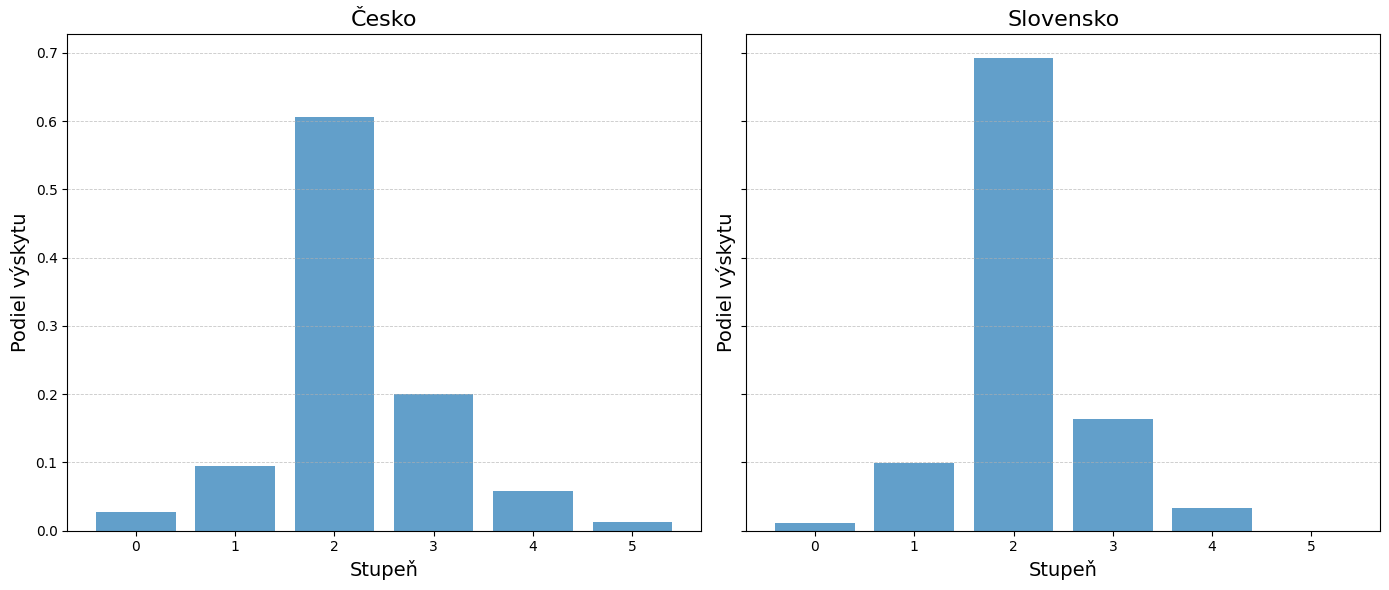
\includegraphics[width=1\textwidth]{images/degree_distrib.png}}
    \caption{Rozdelenie stupňa vrcholov}
    \label{obr:degree_distrib}
\end{figure}

Ako ďalšie si uvedieme porovnanie oboch krajín na základe rôznych centralít.

\textbf{Centralita prepojenosti} - táto metrika nám hovorí o tom na koľko je daný uzol prepojovacím článkom v celej sieti, teda koľko dôležitých ciest cezeň vedie. Formálne pre každý vrchol $v$ definujeme 
\begin{equation*}
    c_B(v) =\frac{\sum_{s,t \in V} \frac{\sigma(s, t|v)}{\sigma(s, t)}}{\frac{(n-1)(n-2)}{2}}
\end{equation*}

kde $V$ je množina uzlov, $\sigma(s, t)$ je počet najkratších ciest medzi $s$ a $t$ a $\sigma(s, t |v)$ je počet týchto ciest, ktoré vedú cez nejaký uzol $v$ odlišný od $s$ a $t$. Ak $s = t$, potom $\sigma(s, t) = 1$, a ak $v \in \{s, t \}$, potom $\sigma(s, t |v ) = 0$. 

\begin{figure}
    \centerline{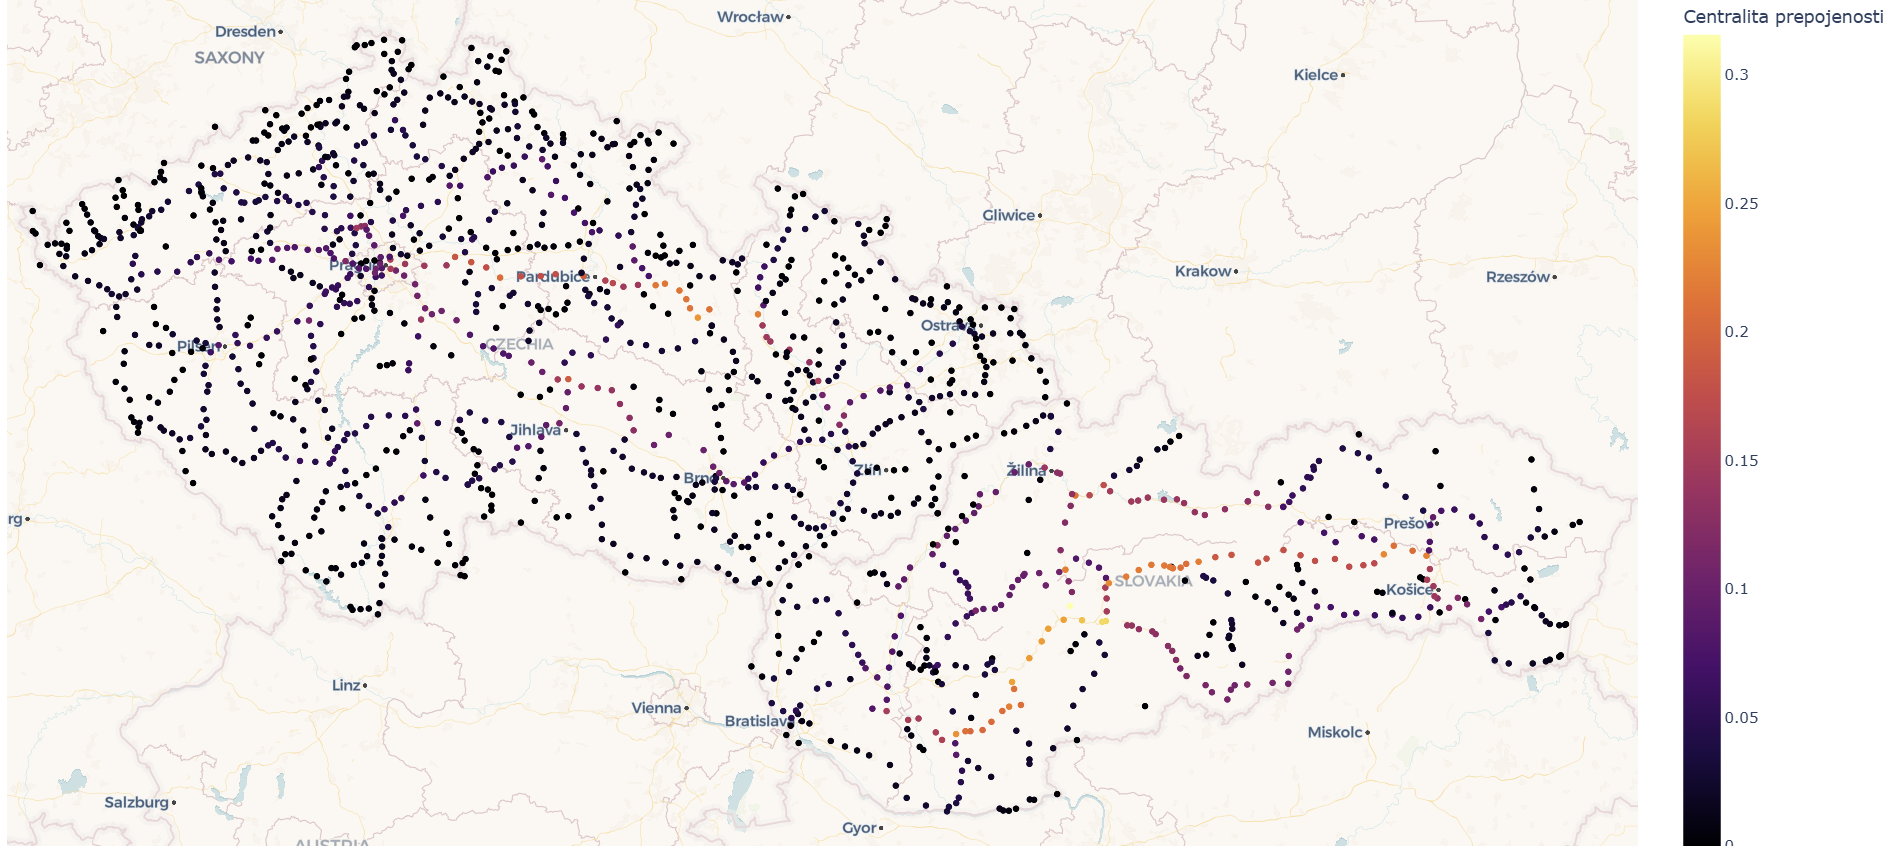
\includegraphics[width=1\textwidth]{images/betweenes.png}}
    \caption{Centralita prepojenosti}
    \label{obr:betweenes}
\end{figure}

Situáciu našich dát možno vidieť na obrázku \ref{obr:betweenes}. Najdôležitejšie stanice z hľadiska centrality prepojenosti na Slovensku sa nachádzajú na „strednej“ trati, konkrétne na úseku vedúcom z Nových Zámkov cez Banskú Bystricu až do Prešova. Tento trend je očakávaný, keďže „vrchná“ a „spodná“ trať sú oproti nej obchádzkovejšie a teda menej priame. V Česku pozorujeme podobný vzor: kľúčové uzly sa sústreďujú v strednej časti republiky, napríklad na trasách z Prahy cez Pardubice alebo z Prahy južnejšie smerom do Brna.

\textbf{Katzova centralita} - metrika, ktorá rožširuje ideu centrality vlastného vektora tak, že berie do úvahy nielen priame susedstvá,  ale aj všetky dlhšie cesty v grafe, pričom príspevok každej cesty klesá s jej dĺžkou. Pre vrchol $i$ ju definujeme ako:
\begin{equation*}
    x_i = \alpha \sum_{j} A_{ij} x_j + \beta,
\end{equation*}

kde $A$ je matica susedností s vlastnými hodnotami $\lambda$.
Parameter $\beta$ určuje počiatočnú hodnotu centrality a platí
\begin{equation*}
    \alpha < \frac{1}{\lambda_{\max}}.    
\end{equation*}

Pre parameter $\beta$ sme zvolili hodnotu $1$ a $\alpha$ sme nastavili na $\frac{0.8}{\lambda_{max}}$. Na obrázku \ref{obr:katz} môžeme vidieť výsledky pre obe krajiny.

\begin{figure}
    \centerline{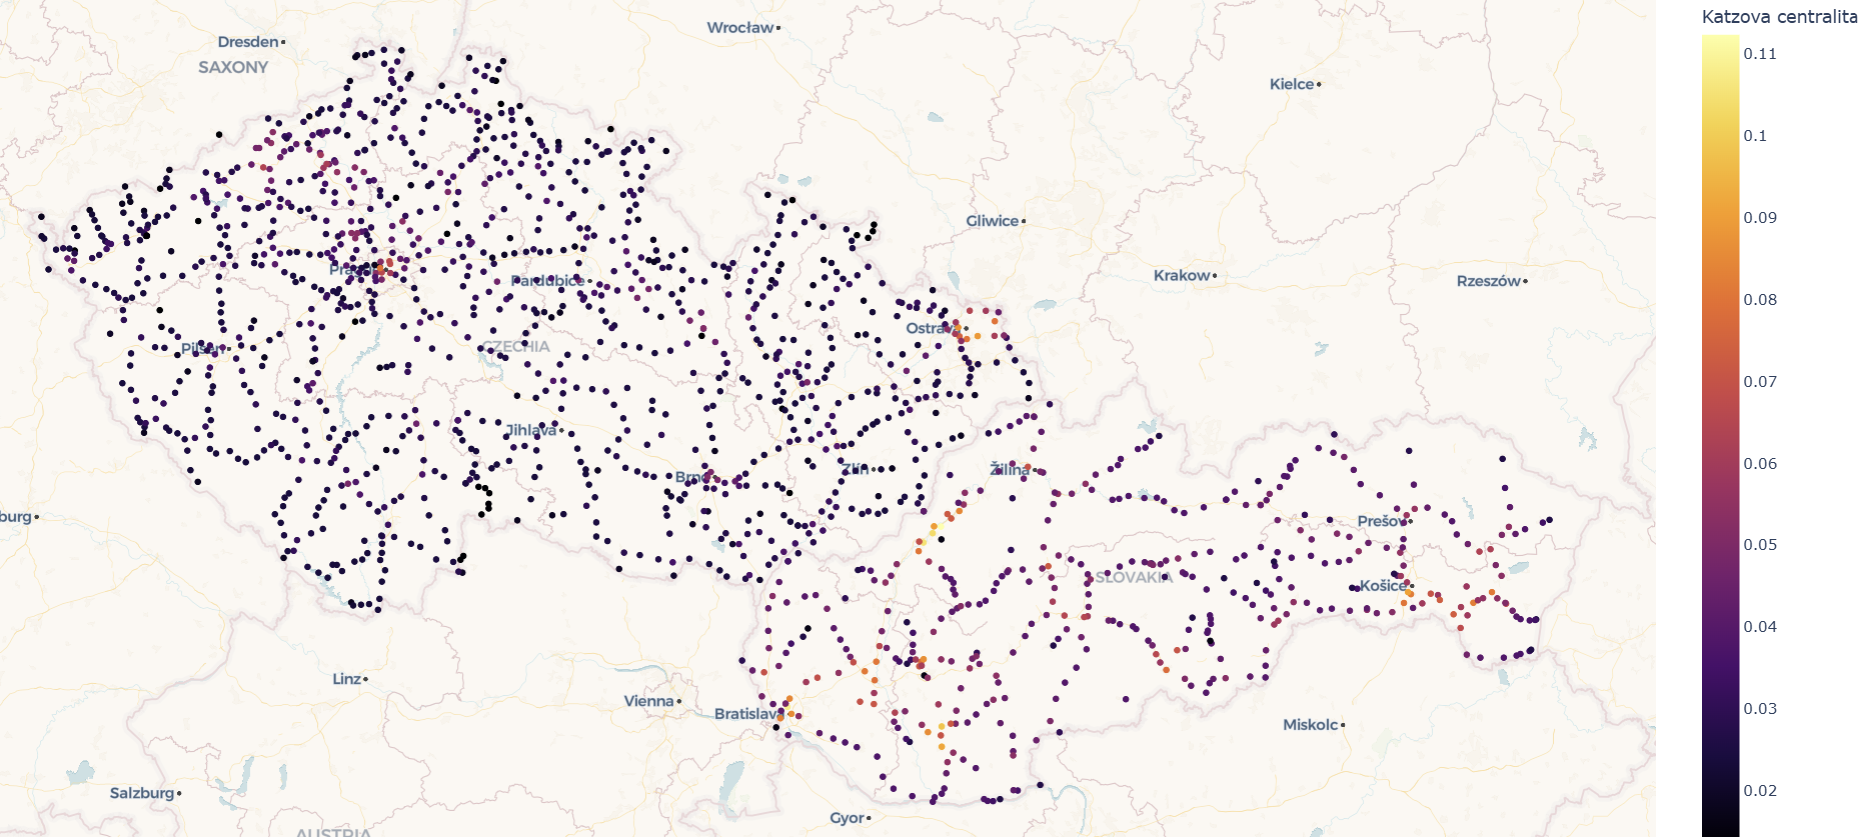
\includegraphics[width=1\textwidth]{images/katz.png}}
    \caption{Katzova centralita}
    \label{obr:katz}
\end{figure}

Vidíme, že pre Slovensko aj Česko sa ukazujú dôležité stanice v hlavných mestách. Na Slovensku sa však tentokrát javí ako dôležitá \uv{vrchná} trať vedúca cez Trenčín. \#NOTE neviem dalej... mozno toto cele vyhodit?

Ako posledné sa pozrieme na skupiny vrcholov a to v južnej a severnej časti krajiny, keďže trate sa zdajú byť celkom odseparované. Sieť si najprv rozdelíme na severnú a južnú časť, tak ako na obrázku \ref{obr:split}.

\begin{figure}
    \centerline{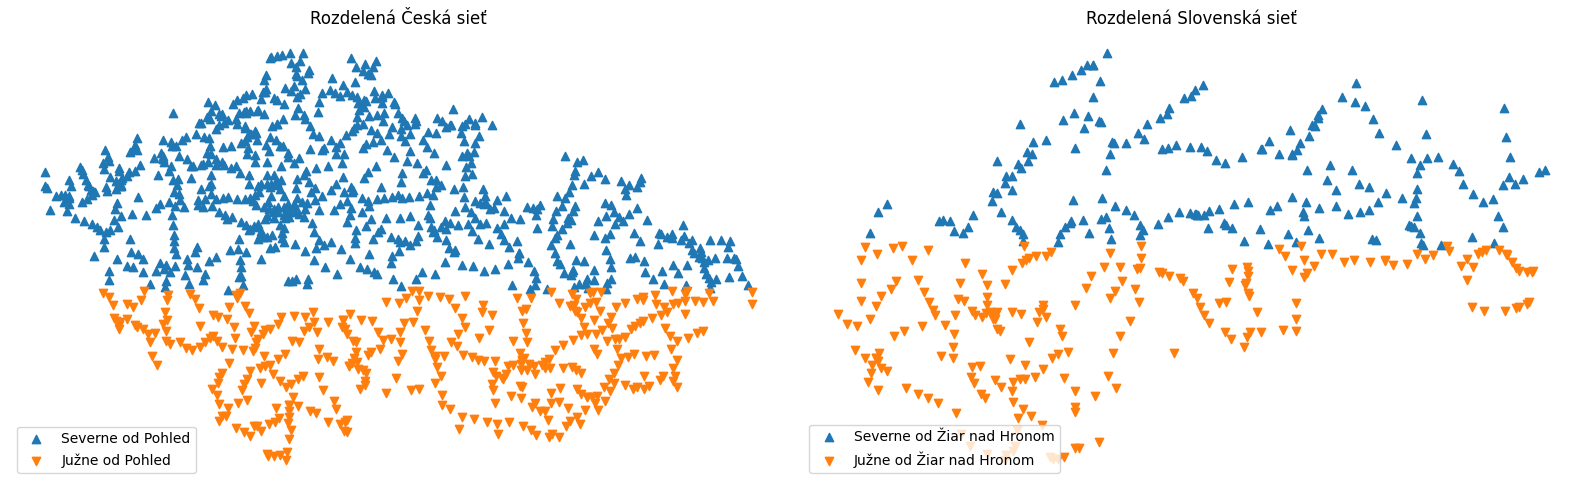
\includegraphics[width=1\textwidth]{images/south_north_split.png}}
    \caption{Rozdelenie na južnú a severnú časť pre obe krajiny}
    \label{obr:split}
\end{figure}

Pre takto rozdelenú sieť spočítame modularitu vzhľadom na príslušnosť ku danej skupine. Váženú modularitu vzhĺadom na nezoraditeľnú vlastnosť definujeme takto: 
 \[
Q_w \;=\;
\frac{1}{2m}
\sum_{i,j}
\Bigl(
  w_{ij}
  - \frac{k_i\,k_j}{2m}
\Bigr)
\;\delta_{g_i,g_j},
\]
kde
\[
k_i = \sum_j w_{ij},
\qquad
m = \frac{1}{2}\sum_{i,j}w_{ij},
\qquad
\delta_{g_i,g_j} =
\begin{cases}
1, & g_i = g_j,\\
0, & \text{inak.}
\end{cases}
\]

Vyšli nám hodnoty $0.96$ pre Češko a $0.90$ pre Slovensko čo znamená, že väčšina váhy, teda kilometrov trate sa nachádza vnútri daných skupín. Prekvapivo pre Česko je to o $6\%$ viac ako pre Slovensko, čo by sme nemuseli očakávať, keďže na obrázku \ref{obr:split} vidíme, že vrcholy sú bližšie pri sebe na nami zadefinovanej hranici oddeľujúcej \uv{juh} a \uv{sever}.
\end{document}

